\chapter{Design And Implementation}
% - Design and Implementation
%   - overview
%   - original tinkering and considerations
%   - features and considerations
%       - readline
%       - golang
%       - logging
%           - remote phoning home
%       - extensibility (markdown, parser)
%       - embedded files
%           - Template expansion
%           - Running examples
%       - usability 
%   - architecture of cli-tool
%   - architecture of web-tool
%       - how sandboxing is achieved
\label{chap:design}
\section{Overview}
% Libs and tools used

\subsubsection{sub}

\subsubsection{Anatomy of a lesson} A lesson is a container that contains a
series of tasks. A lesson has a title and description which are used to
populate the menu screen of \textit{CLI-Tutor}. Every task contains a title and
description as well. The title of a task is displayed in the task tracker and
the description is the actual textual content of a task. This content is either
explaining a concept to the user, displaying a diagram or prompting the user to
input some commands. The amount of tasks dictates the length of the lesson. The
user can keep track of their progress inside a lesson by the task tracker,
which displays the title of the current task as well as a progression counter.

\paragraph{Logging} To assist with gathering usage data and user behaviour,
\textit{CLI-Tutor} maintains a log file which can be optionally sent back to a
server for examination. The log file is a mirror copy of the lesson session
with timestamps for every action that occurs during the lesson.
\section{Architecture}
\section{Extending CLI-Tutor}


\section{Web Application}
\subsection{Overview of Web Application}


\paragraph{Frontend} The frontend is a simple Javascript web application that
presents the user with a special front end terminal component. This component
is then connected to a backend API\footnote{Application Programming Interface}
running on the same server which uses \textit{docker} to create containers on
demand. The containers are then connected to the web terminal (see: \autoref{fig:webversion}) on the frontend
and a WebSocket\footnote{A full-duplex communication protocol native to modern
web browsers.} connection is established to allow the user to interact
with the provisioned \textit{docker} container.

\paragraph{Backend} The backend is a REST\footnote{Representational state
transfer: An architectural style for creating interfaces to allow Client-Server
communication.} API, written in Go. The API allows the frontend to communicate
with the \textit{docker daemon} running on the server, to create,
resize and stop containers on the backend.
 
\paragraph{CLI Only} As mentioned earlier, a CLI only version (see: \autoref{fig:cliversion})was also created
using essentially the same architecture as the version that includes
\textit{CLI-Tutor}. Slight visual differences were made to differentiate the
two however they are based on fundamentally the same \textit{docker} image, with
the only difference being that the "CLI Only" version does not contain the
\textit{CLI-Tutor} tool and drops the user directly into a Linux shell.

\paragraph{Documentation Website} Created using MkDocs,\cite{mkdocs} a widely
used tool for documentation in the software development world. The
documentation website (see: \autoref{fig:docsweb}) was also built to support the
User Study. It uses the same lessons as in the \textit{CLI-Tutor}
application, albeit with some prompts for user interface actions removed.
\begin{lstlisting}[float=htbp, frame=single, language={}, label=lst:markdown, caption=Specification for Markdown lesson files.]
# Lesson Title

A line under a level 1 heading is the lesson description. This is also
displayed in the menu.

## First Task Title

Task instructions are parsed as normal lines under a level 2 heading.

Even line breaks and nested elements will reflect in the lesson. This greatly
enhances readability.

`Commands` are highlighted with backticks.

Text can be injected into a lesson at the time of parsing with template
functions like this --> {{SomeFunc}}

## Second Task Title

This is the first line following a second level 2 heading and thus the text of
task #2.

```
Code blocks can also be used to represent larger blocks of instructions or for
ASCII diagrams.
```
## Interactive tasks with expected values

If the current task is expecting a certain output to a command the user types,
we can specify that using the `>` syntax.

> {{TestFunc}}

## Runtime expected value calculation

Sometimes the correct value for a given task can only be computed at run time,
to achieve this we can specify the expected value of a task to be the output of
a system call by prepending a `!` and then the expected command.

> !ls -la

### Lesson Vocabulary (Provided as a comma separated list of values under a
level 3 heading )

vim, ls, cp, cat, echo <--- only these commands will be permitted in this lesson.

\end{lstlisting}

\subsubsection{Subsubsection}

\paragraph{Paragraph.} Always with a point.


\begin{figure}[htbp]
	\centering
	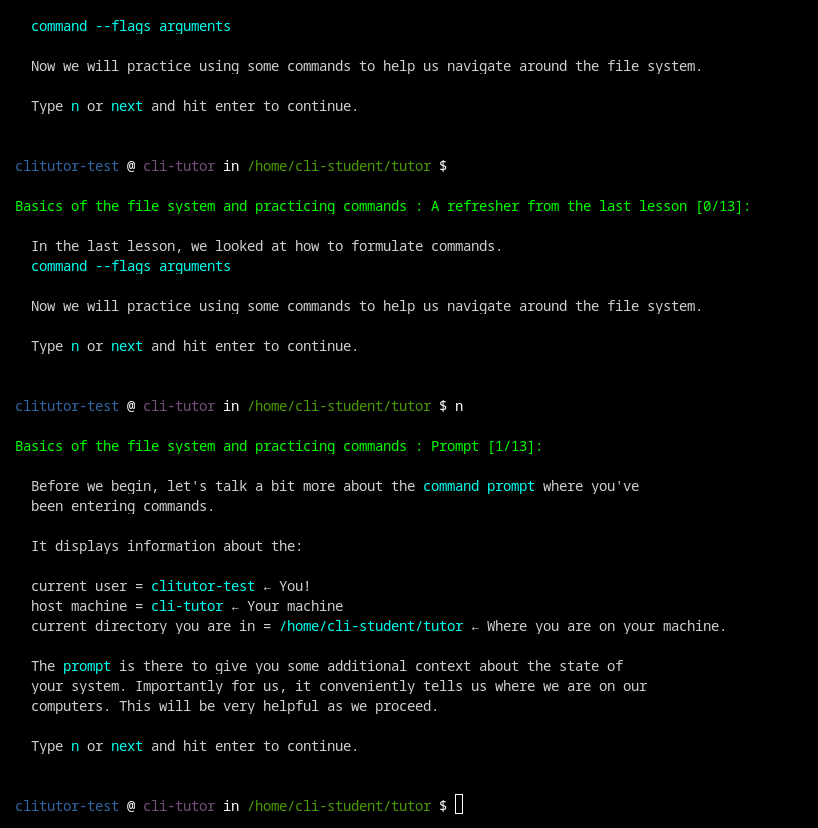
\includegraphics[width=1\textwidth]{img/cliexpansionfull}
	\caption{Screen shot of a \textit{CLI-Tutor} lesson showing values interpolated into the lesson.}
	\label{fig:templateexpansion}
\end{figure}
